\chapter{Signaux et systèmes}
\begin{wrapfigure}[5]{r}{5.5cm}
\vspace{-5mm}
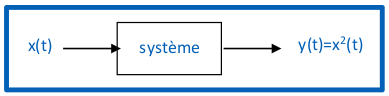
\includegraphics[scale=0.45]{ch1/image1.png}
\captionof{figure}{Exemple de système}
\end{wrapfigure}
Un \textit{signal} représente une information concernant le comportement ou l'état 
d'un phénomène. Ce signal est représenté mathématiquement par une fonctions. Un 
\textit{système} agit sur des signaux d’entrée et produit, à sa sortie, des signaux 
sous une forme plus appropriée pour l’utilisation envisagée.

\section{Signaux}
Il existe deux types de signaux
\begin{enumerate}
\item \textit{A temps continu} ; fonction $f(t)$ est définie pour toute valeur de 
la variable indépendante $t$.
\item \textit{A temps discret}\footnote{ou \textit{signal échantillonné}} ; fonction 
définie seulement pour des valeurs discrète de la variable indépendante. Il s'agit 
par exemple d'une suite de valeurs $\mathbb{R}$ ou $\mathbb{C}$ 
\begin{equation}
x(n),\qquad n \in\mathbb{N}
\end{equation}
\end{enumerate}

\begin{wrapfigure}[8]{l}{7.5cm}
\vspace{-10mm}
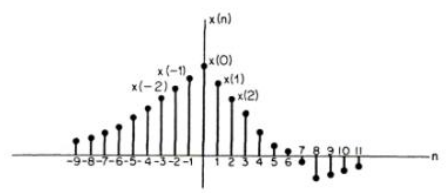
\includegraphics[scale=0.45]{ch1/image2.png}
\captionof{figure}{ }
\end{wrapfigure}
Souvent, on procède à un \textit{échantillonnage} d'un signal à temps continu (TC) pour 
obtenir un signal à temps discret (TD) 
\begin{equation}
x(n) = f(nT)
\end{equation}
où $x$ est discret, $f$ continu et $T$ est la période d’échantillonnage.\\

Le signal à TD se distingue du signal à TC par la \textit{quantification} de sa variable 
indépendante ($t$). On pourrait également envisager la quantification de l'amplitude : un 
signal est dit \textit{numérique} lorsque $t$ et l'amplitude sont quantifiées et 
\textit{analogique} lorsque ces deux valeurs évoluent de façon continues.

	\subsection{Signaux déterministes ou aléatoires}
	Dans un signal \textit{déterministe}, l'évolution en fonction du temps (ou de la 
	variable indépendantes) est à priori connue. Par contre, l'évolution temporelle
	\footnote{Je considère que la variable indépendante sera le temps dans ce chapitre.} 
	d'un signal \textit{aléatoire}.
	
	\subsection{Signaux à énergie finie et signaux à puissance moyenne finie}
	\subsubsection{Signaux à énergie finie}
	L'énergie et la puissance d'un signal $x(t)$ sur $t \in [t_1;t_2]$ est donnée par 
	(le module permet la généralisation aux fonction complexes)
	\begin{equation}
	E(t_1,t_2) = \int_{t_1}^{t_2} |x(t)|^2\ dt,\qquad
	P(t_1,t_2) = \dfrac{1}{t_2-t_1}\int_{t_1}^{t_2} |x(t)|^2\ dt
	\end{equation}
	L'énergie du signal à TC sera dite finie si
	\begin{equation}
	E \int_{-\infty}^{+\infty} |x(t)|^2\ dt < \infty
	\end{equation}
	Pour le signal $TD$, il suffit de remplacer $\int_{-\infty}^{+\infty}$ par 
	$\sum_{-\infty}^{+\infty}$.\\
	La puissance moyenne totale de tels signaux est nulle : ils sont de types 
	transitoires et les seuls physiquement accessibles.
	
	\subsubsection{Signaux à puissance moyenne finie}
	La puissance moyenne finie (TC et TD) pour un signal $x$
	\begin{equation}
	P = \lim\limits_{T\rightarrow\infty} \dfrac{1}{2T}\int_{-T}^T |x(t)|^2\ dt,\qquad
	P = \lim\limits_{N\rightarrow\infty} \dfrac{1}{2N+1}\sum_{-T}^{+N} |x(n)|^2
	\end{equation}
	est bornée et non nulle ($0<P<\infty$). Dès lors, l'énergie de ces signaux est 
	infinie (signaux périodiques et aléatoires stationnaires). Les signaux à énergie 
	et puissance infinie n'appartiennent à aucune des deux catégories précédentes.
	

\section{Systèmes}	
\begin{wrapfigure}[8]{l}{8.5cm}
%\vspace{-10mm}
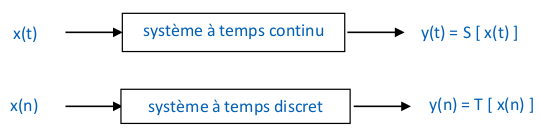
\includegraphics[scale=0.45]{ch1/image3.png}
\captionof{figure}{ }
\end{wrapfigure}
Ceux-ci réalisent la transformations de signaux, on utilise dès lors la même terminologie 
(TC, TD, numérique, analogique). Notons qu'il existe également des structures hybrides. 
On représente un système par un opérateur fonctionnel établissant une règle de correspondance 
entre deux ensembles de fonctions.\\

	\subsection{Caractéristiques de systèmes}
		\subsubsection{Linéarité}
		Un TC/TD est linéaire s'il satisfait au principe de superposition
		\begin{equation}
		S[ax_1(t)+bx_2(t)] = aS[x_1(t)] + bS[x_2(t)],\qquad 
		T[ax_1(n)+bx_2(n)] = aT[x_1(n)] + bT[x_2(n)]
		\end{equation}
		où $a,b\in\mathbb{C}$. Une entrée nulle ($\forall t$ ou $n$) suscite une réponse 
		nulle : $y(n) = 2x(n)+3$ n'est ainsi pas linéaire (waw).
		
		\subsubsection{Permanence (invariance dans le temps)}
		Un système est permanent si un décalage temporel du signal d’entrée produit le même 
		décalage du signal de sortie.
		\begin{itemize}
		\item[$\bullet$ TC ;] $y(t) = S[x(t)]\quad\Rightarrow\quad y(t-t_0) = S[x(t-t_0)]\qquad 
		\forall t_0\in\mathbb{R}$
		\item[$\bullet$ TD ;] $y(t) = T[x(n)]\quad\Rightarrow\quad y(t-k) = T[x(n-k)]\qquad 
		\forall k\in\mathbb{Z}$		
		\end{itemize}
		
		\subsubsection{Causalité}
		Un système est dit \textit{causal} si le signal de sortie à tout instant ne dépend que 
		des valeurs passées et présente du signal d'entrée. On l'exprime
		\begin{itemize}
		\item[$\bullet$ TC ;] \ 
		\begin{itemize}
		\item[*] $x_1(t) = x_2(t)$ pour $t\leq t_0 \quad \Rightarrow\quad y_1(t)=y_2(t)$ pour 
		$t\leq t_0$.
		\item[*] $x(t) = 0$ pour $t\leq t_0\quad \Rightarrow\quad y(t)=0$ pour $t\leq t_0$.
		\end{itemize}
		\item[$\bullet$ TD ;] \ 
		\begin{itemize}
		\item[*] $x_1(n) = x_2(n)$ pour $n\leq n_0 \quad \Rightarrow\quad y_1(n)=y_2(n)$ pour 
		$n\leq n_0$.
		\item[*] $x(n) = 0$ pour $n\leq n_0\quad \Rightarrow\quad y(n)=0$ pour $n\leq n_0$.
		\end{itemize}
		\end{itemize}	
		Notons qu'un système est toujours causal si $t$ (ou $n$) est le temps réel.
		
		\subsubsection{Stabilité}
		Un système est dit stable (au sens strict) si tout signal d'entrée bornée produit 
		une sortie également bornée (stabilité BIBO (bounded input bounded output) :
		\begin{itemize}
		\item[$\bullet$ TC ;] $|x(t)| \leq B_x <\infty\quad \forall t\quad \Rightarrow\quad 
		|y(t)| \leq B_y<\infty\quad \forall t$
		\item[$\bullet$ TD ;] $|x(n)| \leq B_x <\infty\quad \forall n\quad \Rightarrow\quad 
		|y(n)| \leq B_y<\infty\quad \forall n$
		\end{itemize}		
	
	
	
	
	
	
	
	
	
	
	
	
	
	
	
	
	
	
	
	
	
	
	
	
	
	
	
	